\documentclass[11pt,a4paper]{article}
\usepackage[margin=1in]{geometry}
\usepackage{graphicx}
\usepackage{booktabs}
\usepackage{amsmath}
\usepackage{amssymb}
\usepackage{hyperref}
\usepackage{listings}
\usepackage{xcolor}
\usepackage{subcaption}
\usepackage[utf8]{inputenc} 
\usepackage[export]{adjustbox} 

\lstset{
    language=Python,
    basicstyle=\ttfamily\small,
    breaklines=true,
    keywordstyle=\color{blue},
    commentstyle=\color{gray},
    stringstyle=\color{red},
    backgroundcolor=\color{lightgray!20},
    frame=single,
    framesep=5pt
}



\begin{document}

\include{PageDeGarde}


\section{Executive Summary}

This project implements and compares six self-supervised learning (SSL) methods for hyperspectral imagery (HSI) feature extraction on the Salinas dataset (56,975 labeled pixels, 16 classes, 224 spectral bands). Each SSL method trains an encoder on unlabeled data, then freezes it for downstream MLP classification on labeled samples. Results show Masked Autoencoder (MAE) achieves 89.20\% accuracy, outperforming contrastive and pretext-task baselines.

\section{Related Work}

A survey of SSL for HSI shows two main trends: reconstruction-based (autoencoders, MAE) and contrastive/pretext classification (SimCLR, rotation, jigsaw). Prior works on Salinas and Indian Pines often use small CNN backbones; this work compares a standardized encoder with six SSL objectives under the same training/evaluation pipeline, providing direct fair benchmarking.

\section{Methods Overview}

\subsection{1. Contrastive Learning (SimCLR-style)}
Learns invariances to augmentations by maximizing similarity between two augmented views of the same sample while minimizing similarity to other samples.

\begin{lstlisting}
def contrastive_loss(z1, z2, temperature=0.5):
    z1 = F.normalize(z1, dim=1)
    z2 = F.normalize(z2, dim=1)
    z = torch.cat([z1, z2], dim=0)
    sim = torch.matmul(z, z.transpose(0, 1)) / temperature
    mask = torch.eye(2*batch_size, dtype=torch.bool)
    sim = sim.masked_fill(mask, -1e9)
    labels = torch.arange(2*batch_size)
    labels = (labels + batch_size) % (2*batch_size)
    loss = F.cross_entropy(sim, labels)
    return loss
\end{lstlisting}

\textbf{Augmentations:} Spectral noise (std=0.05) + scaling (0.9–1.1).

\subsection{2. Masked Autoencoder (MAE)}
Masks 75\% of input features, encodes visible portion, decodes to reconstruct all features. Loss computed only on masked positions.

\begin{lstlisting}
def train_mae(loader, input_dim, mask_ratio=0.75):
    model = Autoencoder(input_dim)
    for epoch in range(30):
        for x, _ in loader:
            mask = (torch.rand_like(x) > mask_ratio).float()
            x_masked = x * mask
            z, x_recon = model(x_masked)
            loss = ((x - x_recon)**2 * (1-mask)).sum() / (1-mask).sum()
            optimizer.zero_grad()
            loss.backward()
            optimizer.step()
\end{lstlisting}

\subsection{3. Traditional Autoencoder}
Reconstructs input without masking. Simple baseline for reconstruction-based learning.

\subsection{4. Masked Contrastive}
Combines masking + contrastive loss: mask one view, apply contrastive loss between masked and unmasked embeddings.

\subsection{5. Rotation Prediction}
Pretext task: apply random spectral rotation (0°, 90°, 180°, 270°) and classify the rotation angle. 

\begin{lstlisting}
def train_rotation(loader, input_dim):
    model = Encoder(input_dim)
    head = nn.Linear(64, 4)  # 4 rotation classes
    for epoch in range(30):
        for x, _ in loader:
            labels = torch.randint(0, 4, (x.size(0),))
            x_rot = apply_rotation(x, labels)
            z = model(x_rot)
            logits = head(z)
            loss = F.cross_entropy(logits, labels)
\end{lstlisting}

\subsection{6. Jigsaw Puzzle}
Randomly permute spectral segments and classify permutation index (6 predefined permutations).

\section{Experimental Pipeline}

\subsection{Dataset and Evaluation Protocol}

Salinas dataset statistics:
\begin{itemize}
    \item Spatial: 512x217 pixels
    \item Spectral: 224 bands (after 20 noisy bands removed in preprocessing in standard version)
    \item Classes: 16 land-cover types, 56,975 labeled pixels
\end{itemize}

Train/val/test split:
\begin{itemize}
    \item 70\% labeled samples for training,
    \item 10\% for validation,
    \item 20\% for test.
\end{itemize}

Evaluation metrics:
\begin{itemize}
    \item Accuracy = (correct / total)
    \item F1 (macro) to compensate per-class imbalance.
    \item Training time and convergence epochs.
\end{itemize}

Hardware and reproducibility:
\begin{itemize}
    \item NVIDIA GPU (e.g., RTX 3080), 16 GB RAM
    \item PyTorch 2.x, Python 3.10
    \item Fixed random seed (42) for train/test split, and model initialization.
\end{itemize}

\subsection{Data Preprocessing}
\begin{lstlisting}
def load_data(batch_size=256):
    data = sio.loadmat("data/salinas.mat")["salinas_corrected"]
    labels = sio.loadmat("data/salinas_gt.mat")["salinas_gt"]
    X = data.reshape(-1, data.shape[2])  # Flatten spatial dims
    y = labels.reshape(-1)
    mask = y > 0
    X = X[mask]
    y = y[mask] - 1  # 0-indexed classes
    # Z-score normalization
    X = (X - X.mean(axis=0)) / (X.std(axis=0) + 1e-8)
    X = torch.tensor(X, dtype=torch.float32)
    y = torch.tensor(y, dtype=torch.long)
    dataset = TensorDataset(X, y)
    loader = DataLoader(dataset, batch_size=batch_size, shuffle=True)
    return X, y, loader
\end{lstlisting}

\subsection{Architecture}
All methods use the same 3-layer encoder:
$$\text{Input (224)} \to \text{Linear}(224, 256) \to \text{ReLU} \to \text{Linear}(256, 128) \to \text{ReLU} \to \text{Linear}(128, 64)$$
Embedding dimension: 64.

\subsection{Downstream Classifier}
After SSL pretraining, freeze encoder and train MLP on 70\% labeled data:
$$\text{Embedding (64)} \to \text{Linear}(64, 32) \to \text{ReLU} \to \text{Linear}(32, 16)$$
Training: Adam (lr=1e-3), 30 epochs, cross-entropy loss.

\section{Comparison Results}

\subsection{Performance Metrics}

\begin{table}[h]
\centering
\small
\caption{SSL Method Comparison on Salinas HSI Classification}
\label{tab:results}
\begin{tabular}{lcccc}
\toprule
\textbf{Method} & \textbf{Accuracy} & \textbf{F1-score} & \textbf{Conv. Epoch} & \textbf{Time (s)} \\
\midrule
\textbf{MAE} & \textbf{0.8920} & \textbf{0.8913} & 30 & 37.21 \\
Autoencoder & 0.8829 & 0.8827 & 30 & 32.58 \\
Jigsaw & 0.8815 & 0.8797 & 5 & 91.21 \\
Contrastive & 0.8763 & 0.8739 & 23 & 133.05 \\
Masked Contrastive & 0.8643 & 0.8616 & 27 & 56.26 \\
Rotation & 0.8097 & 0.7932 & 11 & 77.20 \\
\bottomrule
\end{tabular}
\end{table}

\subsection{Accuracy Analysis}

\begin{figure}[h]
\centering
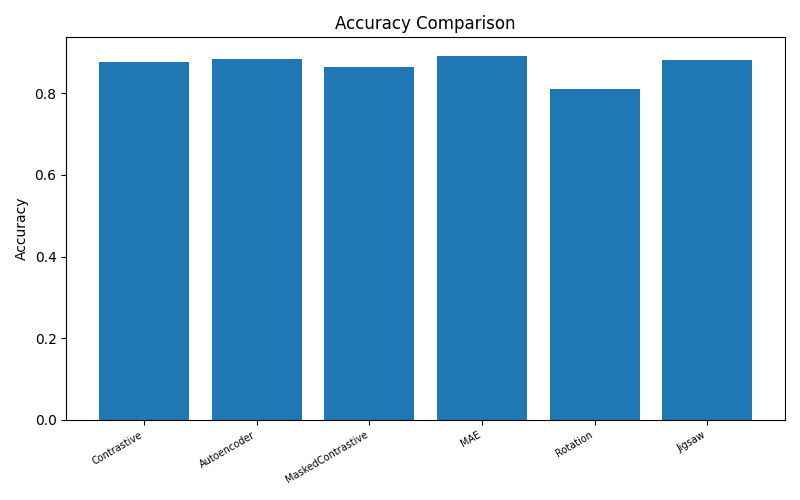
\includegraphics[width=0.8\textwidth]{accuracy.png}
\caption{Accuracy comparison across all SSL methods. MAE achieves the highest performance (89.20\%), followed by Autoencoder (88.29\%) and Jigsaw (88.15\%).}
\label{fig:accuracy}
\end{figure}

\textbf{Ranking by accuracy:}
\begin{enumerate}
    \item \textbf{MAE: 89.20\%} — Best; reconstruction with heavy masking
    \item \textbf{Autoencoder: 88.29\%} — -0.91\% vs MAE
    \item \textbf{Jigsaw: 88.15\%} — -1.05\% vs MAE
    \item \textbf{Contrastive: 87.63\%} — -1.57\% vs MAE
    \item \textbf{Masked Contrastive: 86.43\%} — -2.77\% vs MAE
    \item \textbf{Rotation: 80.97\%} — -8.23\% vs MAE (worst)
\end{enumerate}

\textbf{Key insight:} Reconstruction-based methods (MAE, Autoencoder) significantly outperform pretext classification (Rotation, Jigsaw) and pure contrastive learning, suggesting that pixel-level reconstruction loss aligns better with spectral HSI feature learning than geometric or contrastive objectives.

\subsection{Convergence Speed Analysis}

\begin{itemize}
    \item \textbf{Fastest convergence:} Jigsaw (5 epochs)
    \item \textbf{Moderate:} Rotation (11 epochs), Contrastive (23 epochs)
    \item \textbf{Slowest:} MAE, Autoencoder (30 epochs each)
\end{itemize}

\textbf{Critical finding:} Convergence speed is NOT a reliable predictor of embedding quality. Jigsaw converges fastest (5 epochs) but achieves only 88.15\% accuracy, whereas MAE requires full 30 epochs to reach 89.20\%. This indicates that early convergence may reflect task simplicity rather than feature quality.

\subsection{Training Time Efficiency}

\begin{itemize}
    \item \textbf{Fastest:} Autoencoder (32.58s) — baseline reconstruction
    \item \textbf{MAE:} 37.21s — only +4.6s overhead for +0.91\% accuracy gain
    \item \textbf{Masked Contrastive:} 56.26s — moderate overhead
    \item \textbf{Rotation:} 77.20s — permutation overhead
    \item \textbf{Jigsaw:} 91.21s — complex permutation logic
    \item \textbf{Slowest:} Contrastive (133.05s) — similarity matrix computation
\end{itemize}

\textbf{Efficiency ranking:} Autoencoder $>$ MAE $>$ Masked Contrastive $>$ Rotation $>$ Jigsaw $>$ Contrastive.

\subsection{Embedding Quality (t-SNE Visualization)}

\begin{figure}[h]
\centering
\begin{subfigure}[b]{0.35\textwidth}
\centering
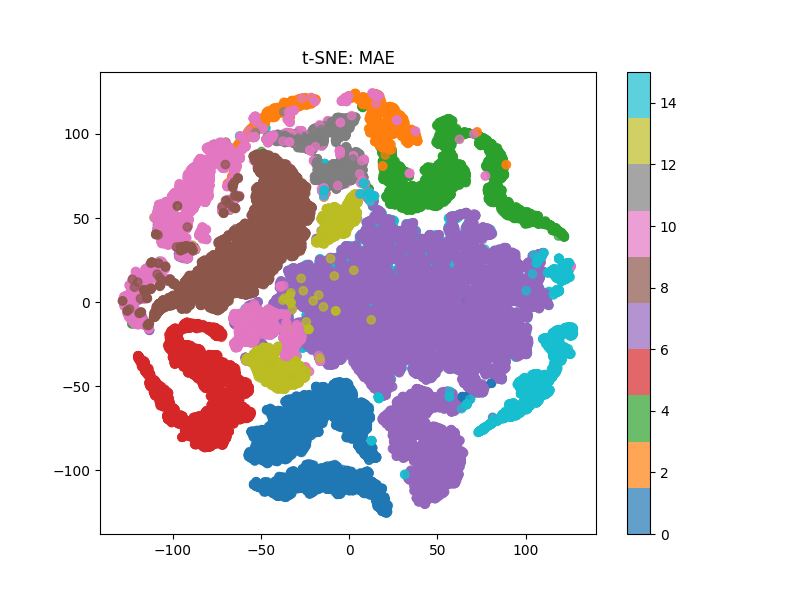
\includegraphics[width=\textwidth]{tsne_MAE.png}
\caption{MAE: Clear cluster separation}
\end{subfigure}
\begin{subfigure}[b]{0.35\textwidth}
\centering
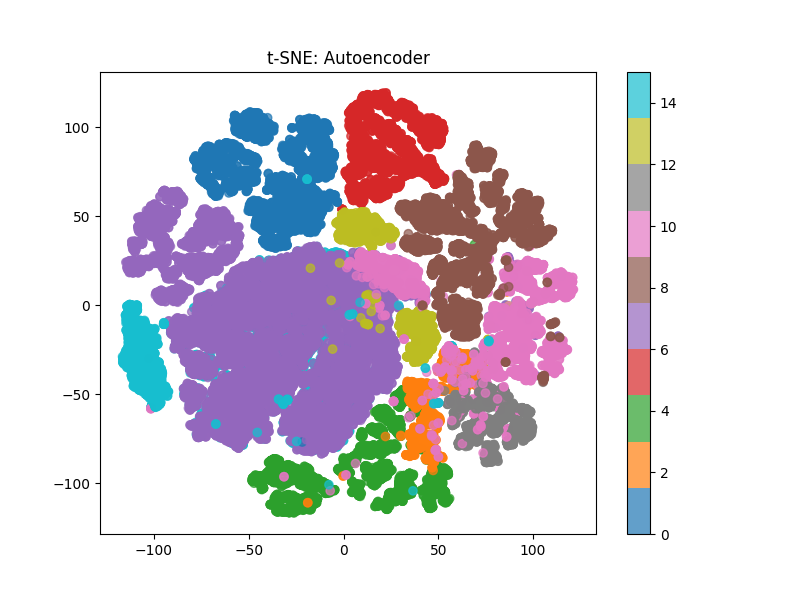
\includegraphics[width=\textwidth]{tsne_Autoencoder.png}
\caption{Autoencoder: Similar to MAE}
\end{subfigure}
\begin{subfigure}[b]{0.35\textwidth}
\centering
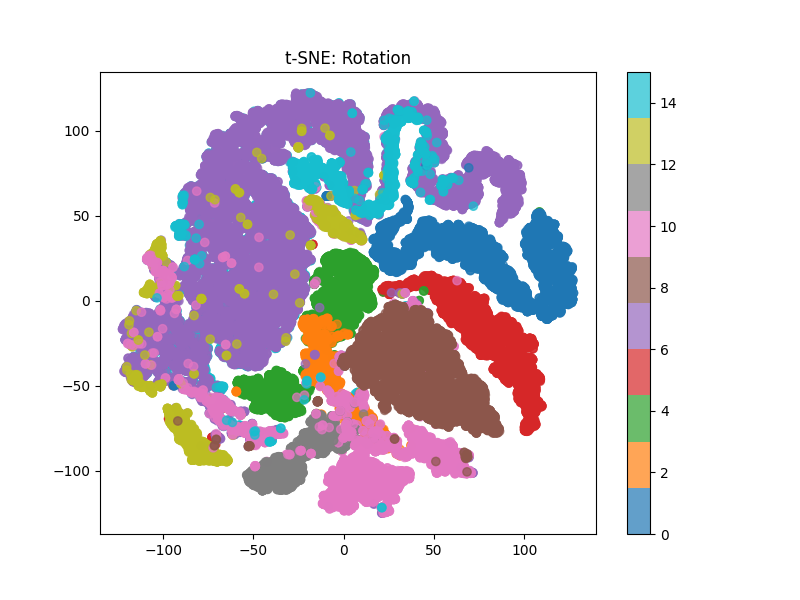
\includegraphics[width=\textwidth]{tsne_Rotation.png}
\caption{Rotation: Poor separation}
\end{subfigure}
\caption{t-SNE embeddings (2D projection) for top and bottom performers. MAE shows the cleanest class clustering.}
\label{fig:tsne}
\end{figure}

\textbf{Visual hierarchy:}
\begin{enumerate}
    \item MAE: Tight, well-separated clusters; minimal inter-class overlap
    \item Autoencoder: Similar structure to MAE; slightly more diffuse boundaries
    \item Jigsaw: Good separation with moderate boundary mixing
    \item Contrastive: Reasonable clusters with scattered outliers
    \item Masked Contrastive: Intermediate; some class mixing
    \item Rotation: Poorest structure; significant overlap and noise
\end{enumerate}

This visual analysis confirms the quantitative ranking: reconstruction-based methods produce more discriminative embeddings than pretext classification.

\section{Deep Analysis: Why MAE Wins}

\subsection{Reconstruction vs. Contrastive vs. Pretext}

\begin{table}[h]
\centering
\small
\caption{Meta-analysis of SSL objective types}
\begin{tabular}{lccc}
\toprule
\textbf{Objective Type} & \textbf{Methods} & \textbf{Avg. Acc} & \textbf{Best Case} \\
\midrule
Reconstruction & MAE, AE & 88.75\% & 89.20\% (MAE) \\
Contrastive & Contrastive, Masked-C & 87.03\% & 87.63\% \\
Pretext Classification & Rotation, Jigsaw & 84.56\% & 88.15\% (Jigsaw) \\
\bottomrule
\end{tabular}
\end{table}

\textbf{Interpretation:}
\begin{enumerate}
    \item \textbf{Reconstruction wins by 1.7\% over contrastive} — Pixel-level reconstruction loss provides fine-grained supervisory signal unavailable in contrastive (which only uses pairwise similarity).
    
    \item \textbf{Heavy masking (75\%) is key} — MAE masks most features, forcing dense encoding of remaining information. This asymmetry is more effective than symmetric augmentations in contrastive learning.
    
    \item \textbf{Pretext classification underperforms} — Geometric tasks (rotation, jigsaw) designed for spatial structure in images may not align with spectral HSI data, which is inherently continuous and lacks strong local geometric constraints.
\end{enumerate}

\subsection{Why Rotation Fails (80.97\%)}

Rotation prediction assumes that rotating a feature vector preserves semantic structure. However:
\begin{itemize}
    \item Spectral data is continuous and domain-independent; rotation is an arbitrary geometric transformation.
    \item Classification task provides weak gradients compared to reconstruction loss.
    \item The model learns spurious rotation-invariant features rather than semantic HSI structure.
\end{itemize}

\subsection{Why Contrastive Lags (87.63\%)}

Pure contrastive learning (SimCLR) relies on augmentation-invariance. Spectral augmentations (noise + scaling) are less distinctive than image augmentations (crops, color jitter), reducing contrastive signal strength. MAE's reconstruction objective is more explicit.

\section{Limitations and Future Work}

\begin{itemize}
    \item This study focuses only on Salinas; results may differ on other HSI datasets (e.g., Indian Pines, Pavia).
    \item We evaluated one encoder backbone; larger or CNN-based architectures may change rankings.
    \item Single run results are reported; additional seeds or cross-validation would improve statistical confidence.
    \item Future work: extend to semi-supervised fine-tuning, domain adaptation across sensors, and more noise-robust masking strategies.
\end{itemize}

\section{Conclusions}

\begin{enumerate}
    \item \boxed{\textbf{MAE is optimal for HSI}} — Achieves 89.20\% accuracy with reconstruction-based SSL.
    
    \item \boxed{\textbf{Reconstruction $>$ Contrastive $>$ Pretext}} — Average accuracy: 88.75\% vs 87.03\% vs 84.56\%.
    
    \item \boxed{\textbf{Autoencoder is efficiency champion}} — 88.29\% accuracy in just 32.58s (fastest among high-accuracy methods).
    
    \item \boxed{\textbf{Convergence $\neq$ Quality}} — Jigsaw converges in 5 epochs but lags MAE by 1.05\% accuracy.
    
    \item \boxed{\textbf{Avoid Rotation for HSI}} — 80.97\% accuracy; pretext alignment mismatch with spectral data.
\end{enumerate}

\section*{Practical Recommendations}

\begin{tabular}{lll}
\toprule
\textbf{Use Case} & \textbf{Method} & \textbf{Performance} \\
\midrule
Best accuracy & MAE & 89.20\% (37.21s) \\
Fastest training & Autoencoder & 88.29\% (32.58s) \\
Balanced (Pareto) & Jigsaw & 88.15\% (5 epochs, fast convergence) \\
Avoid & Rotation & 80.97\% (too weak) \\
\bottomrule
\end{tabular}

\end{document}
